% \iffalse meta-comment
% !TEX program  = pdfLaTeX
%<*internal>
\def\nameofplainTeX{plain}
\ifx\fmtname\nameofplainTeX\else
  \expandafter\begingroup
\fi
%</internal>
%<*install>
\input docstrip.tex
\keepsilent
\askforoverwritefalse
\preamble
--------------------------------------------------------------------------------
AMbeamer <!AMreleaseVersion!> --- AM beamer class
E-mail: romain.pennec@tum.de
Released under the LaTeX Project Public License v1.3c or later
See http://www.latex-project.org/lppl.txt
--------------------------------------------------------------------------------

/!\      Modifications made in this file will be lost!       /!\

\endpreamble
\postamble

Copyright (C) 2003-2010 by S. Lohmeier <lohmeier@amm.mw.tum.de>
Copyright (C) 2011-2013 by M. Schwienbacher <m.schwienbacher@tum.de>
Copyright (C) 2014 by K. Grundl <kilian.grundl@tum.de>
Copyright (C) 2015-2016 by R. Pennec <romain.pennec@tum.de>

This work may be distributed and/or modified under the
conditions of the LaTeX Project Public License (LPPL), either
version 1.3c of this license or (at your option) any later
version.  The latest version of this license is in the file:

http://www.latex-project.org/lppl.txt

This work is "maintained" (as per LPPL maintenance status) by
Romain Pennec.

This work consists of the file  AMbeamer.dtx
and the derived files           AMbeamer.ins,
                                AMbeamer.pdf,
                                beamercolorthemeAM.sty,
                                beamerthemeAM.sty and
                                AMbeamer.cls.

\endpostamble
\usedir{tex/latex/AM/AMbeamer}
\generate{
  \file{\jobname.cls}{\from{\jobname.dtx}{class}}
}
\generate{
  \file{beamercolorthemeAM.sty}{\from{\jobname.dtx}{color}}
}
\generate{
  \file{beamerthemeAM.sty}{\from{\jobname.dtx}{theme}}
}
%</install>
%<install>\endbatchfile
%<*internal>
\usedir{source/latex/AM/AMbeamer}
\generate{
  \file{\jobname.ins}{\from{\jobname.dtx}{install}}
}
\nopreamble\nopostamble
\usedir{doc/latex/AM/AMbeamer}
\ifx\fmtname\nameofplainTeX
  \expandafter\endbatchfile
\else
  \expandafter\endgroup
\fi
%</internal>
\RequirePackage{AMgit}
%<*class>
\NeedsTeXFormat{LaTeX2e}
\ProvidesClass{AMbeamer}[\AMinsertGitDate{} \AMinsertGitVersion{} AM beamer class]
%</class>
%<*driver>
\documentclass{AMdocumentation}
\begin{document}
  \DocInput{\jobname.dtx}
\end{document}
%</driver>
% \fi
%
%
% \changes{1.0}{2015/05/28}{First version}
% \changes{1.5}{2015/11/02}{Beamer part settings}
% \changes{1.5}{2015/11/06}{Tables of contents}
%
%
% \title{The \textcolor{white}{AMbeamer} class}
% \maketitle
% \tableofcontents
%
% \section{License}
% \InsertLicenseBlaBla
%
%
%
% \section{User guide: how to use the AMbeamer class?}
%
% \iffalse
%<*verb>
% \fi
\begin{dispListing*}{usage}
	\documentclass[11pt]{AMbeamer}
\end{dispListing*}
% \iffalse
%</verb>
% \fi
%
%
% \subsection{Class options}
%
% All given options are transfered to parent class \PackageName{beamer}.
%
% \bigskip
%
% \begin{docCommand}{AMsetBeamer}{\marg{option list}}
% Main command for changing the AM settings. 
% \end{docCommand}
%
% \InsertPgfkeysBlaBla{Beamer}
%
% \begin{docKey}[AM/beamer]{fancy maketitle}{}{}
% Command \cs{maketitle} is redefined to the new titlepage version.
% \end{docKey}
%
% \begin{docKey}[AM/beamer]{recall part}{={true/false}}{default \docValue{true}, initially \docValue{false}}
% A frame with the part title will automatically be inserted at every part change
% if you pass this key.
% \end{docKey}
%
% \begin{docKey}[AM/beamer]{recall section}{={true/false}}{default \docValue{true}, initially \docValue{false}}
% A frame with the table of contents title will automatically be inserted at section
% change if you pass this key.
% \end{docKey}
%
% \begin{docKey}[AM/beamer]{recall subsection}{={true/false}}{default \docValue{true}, initially \docValue{false}}
% A frame with the table of contents title will automatically be inserted at subsection
% change if you pass this key.
% \end{docKey}
%
% \iffalse
%<*verb>
% \fi
\begin{dispListing*}{usage}
\AMsetBeamer{fancy maketitle, recall section}
\end{dispListing*}
% \iffalse
%</verb>
% \fi
%
% \subsection{Personalized environments}
%
% \begin{docEnvironment}{theorem}{\oarg{title}}
% Use this environment to insert a theorem.
% It is a standard \PackageName{beamer} environment, redefined with the AM settings.
% \end{docEnvironment}
%
% \begin{docEnvironment}{definition}{\oarg{title}}
% Use this environment to insert a definition.
% It is a standard \PackageName{beamer} environment, redefined with the AM settings.
% \end{docEnvironment}
%
% \begin{docEnvironment}{block}{\marg{title}}
% Use this environment to insert a block. 
% It is a native \PackageName{beamer} environment, redefined with the AM settings.
% \end{docEnvironment}
%
%
% \subsection{Additional frame options}
%
% The following options can directly be used in the beamer environment frame.
%
% \subsubsection{Frame option: grid}
% 
% \iffalse
%<*verb>
% \fi
\begin{dispListing*}{}
\begin{frame}[grid]
content...
\end{frame}
\end{dispListing*}
% \iffalse
%</verb>
% \fi
% 
%
% \subsection{Additional commands}
%
% \subsubsection{Macros of the package}
%
% \begin{docCommand}{AMrecall}{\oarg{graphic options}\marg{picture name}}
% Recall a picture in the top right corner of the frame. Graphic options are
% transfered to the command \cs{includegraphics}. You can use any picture name,
% as long as the corresponding file can be found by latex (you can set the search
% path with the command \cs{graphicspath} of package \PackageName{graphicx})
% \end{docCommand}
%
%
% \begin{docCommand}{sourcepic}{\oarg{options}\marg{picture name}\marg{source}}
% Allows you to add a source label for a picture. It will be added on the picture, by default
% at the bottom right corner. Possible values for the options: (ignore /AM/sourcepic/):
% \begin{itemize}
% \item \refKey{/AM/sourcepic/label color}
% \item \refKey{/AM/sourcepic/label style}
% \item \refKey{/AM/sourcepic/width}
% \item \refKey{/AM/sourcepic/prefix}
% \end{itemize}
% \end{docCommand}
%
% \begin{docCommand}{AMmathboxintheorem}{\oarg{tcb options}}
% Command that you can pass to the \PackageName{empheq} environment.
% \end{docCommand}
%
% \begin{docCommand}{AMmakePartOverview}{}
% Create a frame with an overview of all the parts. This is usefull only for big presentation
% (lecture slides for example), and if you are using \cs{part} of course. 
% See also \refKey{/AM/beamer/recall part}
% \end{docCommand}
%
%
% \subsubsection{Option keys for the macros}
%
% The following options can be set locally or globally. 
%
% \todo{provide an example}
%
% \begin{docKey}[AM/sourcepic]{label color}{=\meta{color name}}{initially \docValue{TUMgrey}}
% Change the color of the picture's source text. Pass this key as option for \refCom{sourcepic}.
% \end{docKey}
%
% \begin{docKey}[AM/sourcepic]{width}{=\meta{picture width}}{initially \docValue{\cs{textwdith}}}
% Total width of the picture. This key is given to \cs{includegraphics}.
% \end{docKey}
%
% \begin{docKey}[AM/sourcepic]{label style}{=\meta{font commands}}{initially \docValue{\cs{scriptsize}}}
% Change the style of the picture's source text, for example the size and the font family.
% \end{docKey}
%
% \begin{docKey}[AM/sourcepic]{prefix}{=\meta{text}}{initially empty}
% This key allows you to add a text before the source label, for example \docValue{\textit{Source: }}
% \end{docKey}
%
%
%
%
%
%
% \newpage
% \setlength{\parskip}{1em}
% \section{Class Implementation}
% 
% \InsertImplementationBlabla
%
%    \begin{macrocode}
%<*class>
%    \end{macrocode}
%
% In order to ensure the compatibility with Adobe Reader (that is not respecting the pdf standards)
% we have to downgrade the pdf version.
% 
%    \begin{macrocode}
\pdfminorversion=4
%    \end{macrocode}
%
%
% \subsection{Load theme}
%
% Package \AMpackage{AMcolor} and \AMpackage{AMfont} are loaded by the AM theme.
%
%    \begin{macrocode}
\LoadClassWithOptions{beamer}
\usetheme{AM}
%    \end{macrocode}
%
% \subsection{Required packages}
%
%    \begin{macrocode}
\RequirePackage{etoolbox}
\RequirePackage{pgfkeys}
\RequirePackage{lmodern}
\RequirePackage{tikz}
\RequirePackage{bookmark}
\RequirePackage{booktabs}
\RequirePackage{csquotes}
\RequirePackage{colortbl}
\RequirePackage{AMref}
\arrayrulecolor{TUMBlue}
%    \end{macrocode}
%
%
% \subsection{Standard infos}
%
% \todo{Use command from package AMlang}
%
%    \begin{macrocode}
\institute{Lehrstuhl f\"ur Angewandte Mechanik \\ Technische Universit\"at M\"unchen}
%    \end{macrocode}
%
% \subsection{Option settings}
% 
%    \begin{macrocode}
\providecommand{\AMset}[1]{\pgfkeys{/AM/.cd,#1}}
\newcommand{\AMsetBeamer}[1]{\pgfkeys{/AM/beamer/.cd,#1}}
%    \end{macrocode}
%
%
% \subsection{Macros parameters}
%
% Declare and initialize keys of the |/AM/sourcepic| family.
%
%    \begin{macrocode}
\pgfkeys{
  /AM/sourcepic/.is family, /AM/sourcepic,
  default/.style={
    label color=TUMgrey,
    width=\textwidth,
    label style={\scriptsize},
    prefix={},
    yshift=0pt,
    },
    label color/.estore in = \AM@sourcepic@label@color,
    label style/.store in = \AM@sourcepic@label@style,
    prefix/.store in = \AM@sourcepic@prefix,
    width/.estore in = \AM@sourcepic@width,
    yshift/.estore in = \AM@sourcepic@yshift,
}
\pgfkeys{/AM/sourcepic,default}
%    \end{macrocode}
%
%
%
% \subsection{Convenient macros}
%
%
% \subsubsection{Depreciated commands}
%
% \begin{docCommand}{bluefat}{\marg{text}}
% Kept for backward compatibility. Should not be used.
% \end{docCommand}
%
%    \begin{macrocode}
\newcommand{\bluefat}[1]{\textbf{\color{TUMblue}#1}}
%    \end{macrocode}
%
%
% \subsubsection{Command sourcepic}
%
% \todo{More options}
%
%    \begin{macrocode}
\newcommand{\sourcepic}[3][]{%
  \pgfkeys{/AM/sourcepic,#1}
  \begin{tikzpicture}
  \node[anchor=south east,inner sep=0] (picture)  {%
    \includegraphics[width=\AM@sourcepic@width]{#2}
  };
  \node[anchor=south east,inner sep=3pt,yshift=\AM@sourcepic@yshift] (source) {%
    \color{\AM@sourcepic@label@color}\AM@sourcepic@label@style\AM@sourcepic@prefix#3
  };
  \end{tikzpicture}
}
%    \end{macrocode}
%
%
% \begin{docCommand}{placepicturetopright}{\oarg{width}\marg{picture name}}
% F. Gruber: Use this code to place a nice figure top right in AMbeamer!!!
% 
% \todo{the name is misleading since this macro can be use to place anything, not only picture.}
% \end{docCommand}
%
%    \begin{macrocode}
\newcommand{\placepicturetopright}[2][0.2\textwidth]{
  \begin{tikzpicture}[overlay, remember picture]
    \node [anchor=north east] at (current page.north east) 
      [xshift=-2mm, yshift=-10mm] {\tiny\def\svgwidth{#1}#2};
  \end{tikzpicture}
}
%    \end{macrocode}
%
%
% \begin{docCommand}{AMput}{\oarg{options}\marg{code}}
% not really working...
% \end{docCommand}
%
%    \begin{macrocode}
\newcommand{\AMput}[2][]{
  \begin{tikzpicture}[overlay, remember picture]
    \node[inner sep=0pt,#1] at (current page) {#2};
  \end{tikzpicture}
}
%    \end{macrocode}
%
% Implementation of \refCom{AMrecall}
%
%    \begin{macrocode}
\newcommand{\AMrecall}[2][width=2cm]{%
  \placepicturetopright{\includegraphics[#1]{#2}}
}
%    \end{macrocode}
%
%
% \begin{docCommand}{AMmove}{\marg{y-translation}\marg{x-translation}\marg{content}}
% Move some content on the frame.
% \end{docCommand}
%
%    \begin{macrocode}
\newcommand{\AMmove}[3]{%
  \vspace{#1}
  \hspace{#2}
  \parbox{\textwidth}{#3}
}
%    \end{macrocode}
%
%
% \begin{docCommand}{gridframe}{\oarg{top right corner}}
%
% Grid for full frame. Little bit hacky in order to fit grid to whole 
% pagewidth with alignment on both sides for the title line... 
% 
% Provided for retro compatibility. Please use option \oarg{grid} of environment
% frame (see next section)
% \end{docCommand}
%
%    \begin{macrocode}
\newcommand{\gridframe}[1][]{%
  \begin{frame}
    \begin{minipage}{\paperwidth}
      \hspace{-6.6mm}
      \begin{tikzpicture}
        \draw[xstep=2.975mm,ystep=2.975mm,color=TUMIvory,line width=0.01pt]
          (0,0) grid (119mm,80.325mm);
        \node[anchor=north east] at (119mm,80mm){\mbox{#1}};
      \end{tikzpicture}
    \end{minipage}
  \end{frame}
}
\let\picgridframe\gridframe
%    \end{macrocode}
%
%
% \subsection{Additional frame options}
%
% The following options can directly be used in the beamer environment frame.
%
%
% \subsubsection{Frame option: grid}
%
% Usage: |\begin{frame}[grid] ... |
% 
%    \begin{macrocode}
\define@key{beamerframe}{grid}[false]{%
\setbeamertemplate{background}
    {
    \begin{tikzpicture}[overlay, remember picture]
        \node [] at (current page.south west) [xshift=12.7pt, yshift=12pt]  
        {\begin{tikzpicture}[remember picture, overlay]
            \draw[xstep=2.975mm,ystep=2.975mm,color=TUMLightGray!80,
            line width=0.01pt](0,0) grid (119mm,80.325mm);
         \end{tikzpicture}
        };
    \end{tikzpicture}
    }  
}
%    \end{macrocode}
%
% Template background is reset at each new frame so that the effect of
% option grid is only local.
%
%    \begin{macrocode}
\pretocmd{\beamer@@@@frame}{\setbeamertemplate{background}{}}{}{}
%    \end{macrocode}
%
%
% \subsection{Boxes}
%
% \begin{docEnvironment}{AMwarning}{}
% \end{docEnvironment}
%
%    \begin{macrocode}
\newenvironment{AMwarning}{%
    \begin{center}
    \textcolor{red}{!!!}
    \hskip1ex
  }{%
    \hskip1ex
    \textcolor{red}{!!!}
    \end{center}
}
%    \end{macrocode}
%
%
% \subsection{Pdf document properties}
%
%    \begin{macrocode}
\AMwritePdfMetaProperties{Created with AMbeamer}
%    \end{macrocode}
%
%
%    \begin{macrocode}
%</class>
%    \end{macrocode}
%
%
%
%
%
%
%
% \section{Color Implementation} 
%
%    \begin{macrocode}
%<*color>
%    \end{macrocode}
%
%
%    \begin{macrocode}
\ProvidesPackage{beamercolorthemeAM}[\AMinsertGitDate{} \AMinsertGitVersion{} AM beamer color theme]
%    \end{macrocode}
%
% Colors are defined in the package \AMpackage{AMcolor}
%
%    \begin{macrocode}
\RequirePackage{AMcolor}
\RequirePackage[many]{tcolorbox}
%    \end{macrocode}
%
%
%
% \subsection{Standard Colors}
%
%
%    \begin{macrocode}
\setbeamercolor{normal text}{fg=black}
\setbeamercolor{alerted text}{fg=red}
\setbeamercolor{example text}{fg=TUMGreen}
\setbeamercolor{structure}{fg=TUMBlue}
%    \end{macrocode}
%
%
%
%
% \subsection{Colors for Frames}
%
%
%    \begin{macrocode}
\setbeamercolor{frametitle}{fg=black}
\setbeamercolor{framesubtitle}{fg=TUMblue}
%    \end{macrocode}
%
%
%
%
% \subsection{Colors of Title Page}
%
%
%    \begin{macrocode}
\setbeamercolor{title}{fg=black}
\setbeamercolor{subtitle}{fg=TUMBlue}
\setbeamercolor{author}{fg=TUMBlue}
\setbeamercolor{institute}{fg=black}
\setbeamercolor{date}{fg=black}
\setbeamercolor{bottom}{fg=TUMDiag6}
%    \end{macrocode}
%
%
%
%
% \subsection{Colors for Boxes}
%
%
%    \begin{macrocode}
\setbeamercolor{TUMbox}{fg=TUMblack,bg=TUMDiag7}
\setbeamercolor{TUMtitle}{fg=white,bg=TUMBlue}
%    \end{macrocode}
%
%
%    \begin{macrocode}
%</color>
%    \end{macrocode}
%
%
%
%
%
%
%
%
% \section{Theme implementation}
%
%    \begin{macrocode}
%<*theme>
%    \end{macrocode}
%
%
%    \begin{macrocode}
\ProvidesPackage{beamerthemeAM}[\AMinsertGitDate{} \AMinsertGitVersion{} AM beamer theme]
\usefonttheme{default}
\usecolortheme{AM}
\useinnertheme{default}
\useoutertheme{default}
%    \end{macrocode}
%
% \begin{docCommand}{AM@emph@color}{}
% Stores the color for the \cs{emph} command.
% \end{docCommand}
%
%    \begin{macrocode}
\def\AM@emph@color{TUMOrange}
\renewcommand{\emph}[1]{\textcolor{\AM@emph@color}{\textit{#1}}}
%    \end{macrocode}
%
% \begin{docCommand}{mathemph}{\marg{math text}}
% Emphasis mathematics.
% \end{docCommand}
%
%    \begin{macrocode}
\newcommand{\mathemph}[1]{\textcolor{TUMBlue}{\mathbf{#1}}}
%    \end{macrocode}
%
%
%
% \subsection{Boxes style}
%
%
%    \begin{macrocode}
\setbeamerfont{example text}{series=\bfseries}
\setbeamerfont{alerted text}{series=\bfseries}
\tcbset{highlight math style={enhanced,arc=0pt,boxrule=0pt,colback=TUMIvory!55}}
%    \end{macrocode}
%
% Implementation of \refCom{AMmathboxintheorem}
%
%    \begin{macrocode}
\newtcbox{\AMmathboxintheorem}[1][]{%
  reset,nobeforeafter,tcbox raise base,
  boxrule=1pt,colframe=TUMGreen,colback=white
  ,arc=0pt,coltext=TUMGreen,#1
}
%    \end{macrocode}
%
%
% \begin{docEnvironment}{AMtheorem}{\oarg{title}}
% Create theorem. 
%todo more details. Show example.
% \end{docEnvironment}
%
%    \begin{macrocode}
\newtcbtheorem[number within=section]{AMtheorem}{}%
{theorem name,highlight math,fonttitle=\bfseries\large,halign title=center,
separator sign none,colbacktitle=white,coltitle=TUMGreen,beforeafter skip=1ex plus 1ex minus .5ex,
titlerule=3pt,colframe=white,width=0.9\textwidth,coltext=TUMBlue}{th}
%    \end{macrocode}
%
%
% \begin{docEnvironment}{AMdefinition}{\oarg{title}}
% Create definition. 
%todo more details. Show example.
% \end{docEnvironment}
%
%
%    \begin{macrocode}
\newtcbtheorem[number within=section]{AMdefinition}{Definition}%
{theorem name,fonttitle=\large,coltitle=TUMBlue,separator sign none,colframe=TUMGreen,empty,
borderline west={1pt}{-10pt}{TUMGreen},blanker,description color=\AM@emph@color,
,description delimiters none,fontupper=\normalfont,oversize}{defi}
%    \end{macrocode}
%
%
% Environment \refEnv{theorem} and \refEnv{definition} 
% are overwritten by \refEnv{AMtheorem} and \refEnv{AMdefinition}.
% 
%    \begin{macrocode}
\setbeamertemplate{theorem begin}
{%
  \empheqset{innerbox=\AMmathboxintheorem}
  \centering
  \def\@tempa{definition}%
  \ifx\@currenvir\@tempa
    \def\AM@usetheorem{AMdefinition}
    \def\AM@emph@color{TUMGreen}
  \else
    \def\AM@usetheorem{AMtheorem}
  \fi
  \begin{\AM@usetheorem}{\inserttheoremaddition}{AMtheoremlabel}
}
\setbeamertemplate{theorem end}{\end{\AM@usetheorem}}
%    \end{macrocode}
%
%
%
% \subsection{Frames style}
%
%
%    \begin{macrocode}
\setbeamerfont{frametitle}{series=\bfseries,size=\Large}
\setbeamerfont{framesubtitle}{series=\itshape,size=\large}
%    \end{macrocode}
%
%
%
% \subsection{Style for titles, footlines, and headlines}
%
%
%    \begin{macrocode}
\setbeamerfont{author}{size=\normalsize, series=\normalfont}
\setbeamerfont{date}{size=\normalsize}
\setbeamerfont{title}{size=\LARGE,series=\bfseries}
\setbeamerfont{subtitle}{size=\large}
\setbeamerfont{section}{series=\bfseries}
\setbeamerfont{institute}{size=\normalsize}
%    \end{macrocode}
%
%
%
% \subsection{Itemize and enumerates}
%
%
% \begin{docCommand}{AM@item@triange}{}
% \end{docCommand}
%
%    \begin{macrocode}
\newcommand{\AM@item@triange}{\raise1.25pt\hbox{\donotcoloroutermaths$\blacktriangleright$}}
\setbeamertemplate{itemize item}{\color{TUMBlue}\scriptsize\AM@item@triange}
\setbeamertemplate{itemize subitem}{\color{TUMGreen}\scriptsize\AM@item@triange}
\setbeamertemplate{itemize subsubitem}{\color{TUMOrange}\tiny\AM@item@triange}
\setbeamertemplate{enumerate item}{\color{TUMGreen}\insertenumlabel.}
\setbeamertemplate{enumerate subitem}{\insertenumlabel.\insertsubenumlabel}
\setbeamertemplate{enumerate subsubitem}{\insertenumlabel.\insertsubenumlabel.\insertsubsubenumlabel}
\setbeamertemplate{enumerate mini template}{\insertenumlabel}
\setbeamertemplate{itemize/enumerate subbody begin}{\normalsize}
%    \end{macrocode}
%
%
%
% \subsection{Navigation symbols}
%
%
%    \begin{macrocode}
\setbeamertemplate{navigation symbols}{}
%    \end{macrocode}
%
%
%
% \subsection{Title page}
%
%
% \begin{docCommand}{TUMtitlepage}{}
% \end{docCommand}
%
%    \begin{macrocode}
\newcommand{\TUMtitlepage}{%
  {%
  \begin{frame}
    \pdfbookmark{\inserttitle}{AMtitleanchor}
    \usebeamerfont{title}
    \usebeamercolor[fg]{title}
    \inserttitle

    \vspace{3 mm}
    \usebeamerfont{subtitle}
    \usebeamercolor[fg]{subtitle}
    \insertsubtitle
   
    \vspace{5 mm}
    \usebeamerfont{date}
    \usebeamercolor[fg]{date}
    \insertdate

    \vspace{10 mm}
    \usebeamerfont{author}
    \usebeamercolor[fg]{author}
    \insertauthor 
  \end{frame}
  }
}
%    \end{macrocode}
%
% \begin{docCommand}{AMbeamer@titleframe}{}
% \end{docCommand}
%
%    \begin{macrocode}
\newcommand{\AMbeamer@titleframe}{
  \begin{frame}[t,plain]
  \vskip1cm
  \begin{tcolorbox}[size=tight,oversize,sharp corners,enhanced,scale=0.5,
    colframe=TUMBlue,colback=TUMBlue,colupper=TUMBlue,
    enlarge left by=-65pt,right=400pt,left=30pt,bottom=30pt,top=20pt,
    frame code app={
    \path[tcb fill frame] ([xshift=-1cm]frame.north) to[out=180,in=0] ([xshift=4cm,yshift=60pt]frame.north west)
      -- ([yshift=60pt]frame.north west) -- (frame.north west) --cycle;
    },overlay={%
    \node[black,anchor=east,xshift=-20pt] at ([xshift=-20pt]frame.east) {
\includegraphics[height=30pt]{AM-logo-TUM-voll-weiss-RGB}};
    \node[black,anchor=west,xshift=32pt,yshift=30pt] at (frame.west) {
\includegraphics[height=75pt]{AM-logo-AM-ivory-RGB}};
    \node[white,xshift=-255pt,yshift=50pt,anchor=west] at (frame.center) {\huge AM};
    \node[white,xshift=-255pt,yshift=25pt,anchor=west] at (frame.center) {\huge Lehrstuhl f\"{u}r};
    \node[white,xshift=-255pt,anchor=west] at (frame.center) {\huge Angewandte Mechanik };
    },overlay app={%
    \node[opacity=1,xshift=-2.0cm] at([xshift=-20pt]frame.east) {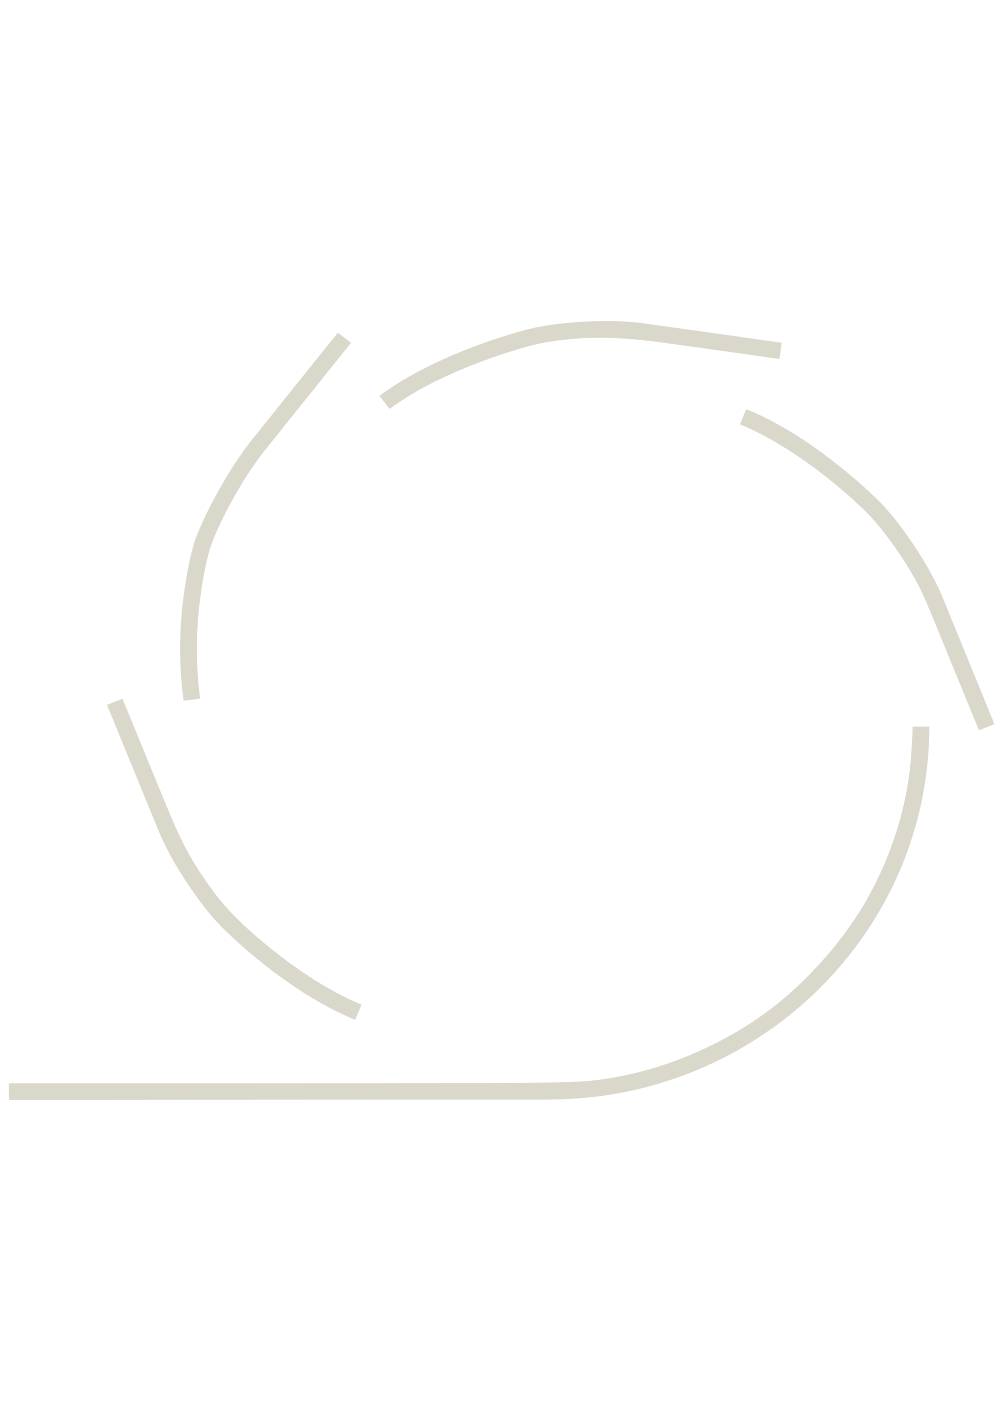
\includegraphics[width=4.5cm]{AM-logo-MW-ivory-RGB}};
    }]
  \end{tcolorbox}
  \vspace{10mm}
  \pdfbookmark{\inserttitle}{AMtitleanchor}
  \usebeamerfont{title}
  \usebeamercolor[fg]{title}
  \inserttitle
  
  \vspace{3mm}
  \usebeamerfont{subtitle}
  \usebeamercolor[fg]{subtitle}
  \insertsubtitle
  
  \vspace{5mm}
  \usebeamerfont{date}
  \usebeamercolor[fg]{date}
  \insertdate
  
  \vspace{10mm}
  \usebeamerfont{author}
  \usebeamercolor[fg]{author}
  \insertauthor 
  \end{frame}
}
%    \end{macrocode}
%
%    \begin{macrocode}
\renewcommand{\maketitle}{\TUMtitlepage}
%    \end{macrocode}
%
%
%
%
%
% \subsection{Header and footer}
%
%
%
% \subsubsection{Header}
%
%
% \cs{pgfdeclareimage} is a command of the package \PackageName{pgfbaseimage}
%
%    \begin{macrocode}
\pgfdeclareimage[width=\paperwidth]{SliceHead}{AM-beamer-slice-head}
\defbeamertemplate*{headline}{standard}
{
  \leavevmode
  \pgfuseimage{SliceHead}
}
%    \end{macrocode}
%
%
%
% \subsubsection{Footer}
%
%
%    \begin{macrocode}
\defbeamertemplate*{footline}{standard}
{
\begin{beamercolorbox}[wd=\paperwidth,ht=2.25ex,dp=1ex,right]{bottom} 
  \vspace*{0pt} \insertframenumber\hspace{1ex}
\end{beamercolorbox} 
}
%    \end{macrocode}
%
%    \begin{macrocode}
\defbeamertemplate*{footline}{titlepage}
{
\begin{beamercolorbox}[wd=\paperwidth,ht=2.25ex,dp=1ex,right]{bottom} 
  % No pagenumber on titlepage
  % \vspace*{0pt} \insertframenumber/5000\hspace{1ex}
\end{beamercolorbox} 
}
\setbeamertemplate{footline}[standard]
%    \end{macrocode}
%
%
%
%
% \subsection{Frametitle and boxes}
%
%
% \todo{check if frame subtitle is given}
%
%    \begin{macrocode}
\setbeamertemplate{frametitle}
{
  \vspace{0.5ex}\hspace{-2.1ex}\parbox{\linewidth}{\insertframetitle}
  \hspace{-2.1ex}\parbox{\linewidth}{%
    \usebeamercolor[fg]{framesubtitle}\usebeamerfont{framesubtitle}
    \insertframesubtitle
  }
}
%    \end{macrocode}
%
%
%
%
% \subsection{Tables of Contents}
%
% Implementation of the following keys:
% \begin{itemize}
% \item \refKey{/AM/beamer/fancy maketitle}
% \item \refKey{/AM/beamer/recall part}
% \item \refKey{/AM/beamer/recall section}
% \item \refKey{/AM/beamer/recall subsection}
% \end{itemize}
%
%    \begin{macrocode}
\newif\ifAM@beamer@toc@current@part
\newif\ifAM@beamer@toc@current@section
\newif\ifAM@beamer@toc@current@subsection
\pgfkeys{
  /AM/beamer/.is family, /AM/beamer,
  recall part/.is if=AM@beamer@toc@current@part,
  recall section/.is if=AM@beamer@toc@current@section,
  recall subsection/.is if=AM@beamer@toc@current@subsection,
  recall part=false,
  recall section=false,
  recall subsection=false,
  fancy maketitle/.code={\renewcommand{\maketitle}{\AMbeamer@titleframe}},
}
%    \end{macrocode}
%
%
% make a frame titled "Outline"
% show TOC and highlight current section
%
% \begin{docCommand}{AM@recall@toc@currentsection}{}
% \end{docCommand}
%
%    \begin{macrocode}
\newcommand{\AM@recall@toc@currentsection}{%
  \begin{frame}<beamer> 
    \frametitle{\hyperlink{AMpartOverview.1}{Outline}}
    \tableofcontents[currentsection]
  \end{frame}
}
\AtBeginSection[]
{
  \ifAM@beamer@toc@current@section\AM@recall@toc@currentsection\fi
}
%    \end{macrocode}
%
%
% \begin{docCommand}{AM@recall@toc@currentsubsection}{}
% \end{docCommand}
%
%    \begin{macrocode}
\newcommand{\AM@recall@toc@currentsubsection}{%
  \begin{frame}<beamer> 
    \frametitle{\hyperlink{AMpartOverview.1}{Outline}}
    \tableofcontents[currentsubsection]
  \end{frame}
}
\AtBeginSubsection[]
{
  \ifAM@beamer@toc@current@subsection\AM@recall@toc@currentsubsection\fi
}
%    \end{macrocode}
%
%
% \begin{docCommand}{AM@create@currentpart}{}
% \end{docCommand}
%
%    \begin{macrocode}
\newcommand{\AM@create@currentpart}{%
  {%
    \addtocontents{toc}{%
      \protect\beamer@partintoc{\the\c@part}{\beamer@partnameshort}{\the\c@page}%
    }%
    \setbeamertemplate{background canvas}{%
      \color{TUMIvory}\rule{\paperwidth}{\paperheight}%
    }%
    \frame{\hypertarget{part:\the\c@part}\partpage}%
  }%
}
\AtBeginPart{%
  \ifAM@beamer@toc@current@part\AM@create@currentpart\fi
}
%    \end{macrocode}
%
%
%
% Implementation of \refCom{AMmakePartOverview}
%
%    \begin{macrocode}
\newcommand{\AMmakePartOverview}{
  \begin{frame}
    \pdfbookmark[1]{Overview}{AMpartOverview}
    \tableofcontents[onlyparts]
  \end{frame}
}
%    \end{macrocode}
%
% \begin{docCommand}{beamer@partintoc}{\marg{part number}\marg{label}\marg{part title}}
% \end{docCommand}
%
%    \begin{macrocode}
\providecommand\beamer@partintoc[3]{%
  \ifnum\c@tocdepth=-1\relax
    \makebox[6em]{\color{TUMOrange} \partname~#1:} \hyperlink{part:#1}{#2}
    \par\vfill
  \fi
}
%    \end{macrocode}
%
% Option key \docValue{onlyparts} for command \cs{tableofcontents}
%
%    \begin{macrocode}
\define@key{beamertoc}{onlyparts}[]{%
  \c@tocdepth=-1\relax
}
%    \end{macrocode}
%
%
%
%    \begin{macrocode}
%</theme>
%    \end{macrocode}
%
%
%
%
%
%
% \Finale
